\documentclass[spanish,a4paper,12pt]{report}
\usepackage[dvips]{graphicx}
\usepackage[dvips]{epsfig}
\usepackage[spanish]{babel}
\usepackage[utf8]{inputenc}
\usepackage{amsmath}
\usepackage{amssymb}
\usepackage{pifont}


\begin{document}
\begin{center}

\includegraphics[width=0.35\textwidth]{logoULL.eps}\\[2mm]
\end{center}


\begin{center}

  {\textbf{\huge{Función de distribución. Hipergeométrica}}}\\[10mm]
  {\Large Adriana Calvo - Misael Enrique Peraza Luis - Carolina Yanes Rivero}\\[3.5mm]
  \textit{Técnicas Experimentales. $1^{er}$ curso. $2^{do}$ semestre}\\[2.5mm]
  \textit{Grupo 3F}\\[2.5mm]
  {Facultad de Matemáticas}\\[2.5mm]
  {Universidad de la Laguna}\\[2.5mm]
  {La Laguna \Today}

\end{center}


\renewcommand{\thepage}{\roman{page}}
\setcounter{page}{1}

\newpage
\begin{abstract}
El propósito de esta exposición consiste en describir de manera objetiva los distintos procedimientos y herramientas utilizadas para llevar a cabo la implementación de la función de distribución de la variable aleatoria hipergeométrica en Python. 

El objetivo principal de este proyecto consiste en aprender a manejar un lenguaje de programación denominado Python, además de usarlo como una herramienta básica en el ámbito matemático. En este trabajo también se encuentran otros objetivos como el de familiarizarse con $\LaTeX$ y Beamer, herramientas básicas en la redacción y exposición de informes y proyectos.
\end{abstract}

\pagebreak

\tableofcontents
\pagebreak

\renewcommand{\thepage}{\arabic{page}}
\setcounter{page}{1}

\chapter{\textbf Motivación y objetivos}


Durante el curso se han visto diferentes métodos matemáticos con el fin de entenderlos y hacer uso de ellos, formulando programas en Python que permitan usarlos de una manera más rápida,sencilla y eficaz. Con este trabajo se pretende profundizar en el aprendizaje de $\LaTeX{}$, Beamer y Python utilizando un tema relacionado con el campo de las matemáticas, en este caso de la \textit{función de distribución} de la variable aleatoria \textbf{hipergeométrica}. Se explicará en que consiste, se dará un código de programación de Python para hacer uso de este método y se comprobará que dicho programa sirve con un ejemplo.

En el subcampo matemático de la probabilidad, la distribución de variable aleatoria hipergeométrica trata de medir el número de éxitos cuando se extrae una muestra de tamaño $n$ sin reemplazamiento.

\pagebreak


\chapter{\textbf Fundamentos teóricos}



Llamamos {\textbf{variable aleatoria}} a toda función que asocia a cada elemento del espacio muestral $\Omega$ $\footnote{Conjunto de todos los posibles resultados individuales de un experimento aleatorio. Cada posible resultado se denomina suceso}$ un número real.

Se utilizan letras mayúsculas $X$, $Y$, ... para designar variables aleatorias, y las respectivas minúsculas ($x$, $y$, ...) para designar valores concretos de las mismas.
Antes de seguir hablando de las variables aleatorias, definamos dos conceptos que nos ayudarán más adelante:
\begin{itemize}

\item{\textbf{Esperanza:} Dice aproximadamente mediante una media las probabilidades de una variable aleatoria.}
\item{\textbf{Varianza:} Muestra la variabilidad de una distribución, indicando por medio de un número, si las diferentes puntuaciones de una variable están muy alejadas de la media. Cuánto mayor sea ese valor, mayor será la variabilidad, cuanto menor sea, más homogénea será a la media. Así se sabe si todos los casos son parecidos o varían mucho entre ellos.}
\end{itemize}

\section{\textbf{Variables aleatorias}}


\subsection{Variable aleatoria continua}
Una variable aleatoria continua es aquella que puede tomar todos los valores posibles dentro de un cierto intervalo de la recta real. \\

{\textit{Altura de los alumnos de una clase, horas de duración de una pila,…}}

\subsection{Variable aleatoria discreta}


Una variable aleatoria discreta es aquella que sólo puede tomar valores enteros. 
\ \\

{\textit{Número de hijos de una familia, puntuación al lanzar un dado,…}}\\
\ \\
Cada variable aleatoria discreta tiene una función de probabilidad o distribución que se denota:\\
 
\centerline{$P_\xi (k) = P({\omega \in \Omega / \xi(\omega) = k}) , \forall k \in \mathbf{N}$}
\ \\
Continuando con este tipo de variable aleatoria, existen diferentes tipos:
\ \\
\begin{itemize}
\item Uniforme
\item Bernouilli
\item Binomial
\item Binomial Negativa
\item Poisson
\item Geométrica
\item Hipergeométrica
\end{itemize}

\section{Variable aleatoria hipergeométrica :}
Dados $N$, $A$ y $B$  números naturales, se llama {\textbf{variable aleatoria hipergeométrica}} de parámetros ($n$ ,$A$ ,$B$) a una variable que trata de medir el número de ''éxitos'' cuando se extrae una muestra de tamaño $n$ sin reemplazamiento. Su función de probabilidad es:\\

\centerline{$P[\xi = k] = \frac {\binom {A} {k} \binom {B} {n-k}} { \binom {N} {n} }$}
\ \\
$\forall k=0,1,…,n$ y se denota por $\xi \sim H(n ,A ,B)$. Se tiene que:\\
\ \\
$E[\xi] = n \cdot \frac{A}{N}$\\
\ \\
$V(\xi) = n \cdot \frac{A}{N} \cdot \frac{B}{N} \cdot \frac{N-n}{N-1}$\\ 

\chapter{\textbf Procedimento Experimental}
\section{Descripción de los experimentos}
Partiendo de la función de distribución hipergeométrica:
\ \\
\centerline{$P[\xi = k] = \frac {\binom {A} {x} \binom {B} {n-x}} { \binom {N} {n} }$}
$A + B = N$
\ \\
Aplicándola a dos ejemplos en particular:

De una baraja española de 40 cartas se extraen 5 al azar. Calcúlese la probabilidad de obtener:
\subsection{Poker de Ases}
\textbf{Poker de Ases :} 4 cartas con el mismo valor de la extracción.\\ 

Se clasificará la baraja en dos grupos, uno con 4 ases, y otro con las 36 cartas restantes que no son as.
Sea la variable $\xi$ (número de ases obtenidos en la extracción de 5 cartas), que se distribuye según la ley hipergeométrica.\\ 
Denominando:\\


\begin{itemize}
\item{$N_1$ = Número de ases en la baraja.}
\item{$N_2$ = Número de no ases en la baraja.}
\item{$N=N_1 + N_2$ = Número de cartas en la baraja.}
\item{$n$ = Número de cartas extraídas de la baraja.}
\item{$x$ = Número de ases en las 5 extracciones.}
\item{$n-x$ = Número de cartas extraídas no ases.}
\end{itemize}

\subsection{Color}
\textbf{Color :} La ''mano'' del mismo palo.\\

Teniendo en cuenta que son 4 palos diferentes. Se denomina:\\

\begin{itemize}
\item{$N_1$ = Número de cartas de un determinado palo.}
\item{$N_2$ = Número de cartas de los otros tres palos.} 
\item{$N=N_1 + N_2$ = Número de cartas en la baraja.}
\item{$n$ = Número de cartas extraídas de la baraja.}
\item{$x$ = Número de cartas extraídas de un determinado palo.}
\item{$n-x$ = Número de cartas extraídas de los otros tres palos.}
\end{itemize}

\section{Descripción del material}
En esta sección se mostrará el material utilizado, es decir, los datos de la máquina:
\begin{itemize}
\item Linux PROA 3.2.0-40-generic 64-Ubuntu SMP Mon Mar 25 21:22:26 UTC 2013 i686 i686 i386 GNU/Linux
\item Python 2.7.3
\item ('default', 'Aug  1 2012 05:16:07')
\item Intel(R) Core(TM)2 Duo CPU     T7250  @ 2.00GHz
\item GenuineIntel
\item 800.000 Hz
\item 2048 KB
\end{itemize}
%%%%%%%%%%%%%
\section{Resultados obtenidos}


Para el poker de ases, se tiene que:

\centerline{$P(\xi=x)=\frac {\binom {N_1} {x} \binom {N_2} {n-x}} { \binom {N} {n} }$}

que, en este caso, se traduce en:
\ \\

\centerline{$P(\xi=4)=\frac {\binom {4} {4} \binom {36} {1}} { \binom {40} {5} }=0,000055$}
\ \\



Para el color la probabilidad de sacarlo de un determinado palo será:
\ \\

\centerline{$P(\xi=5)=\frac {\binom {10} {5} \binom {30} {0}} { \binom {40} {5} } = 0.000383$} 

\ \\

donde $\xi$ es la variable (número de cartas extraídas de un determinado palo).\\
Pero como la baraja tiene cuatro palos, la probabilidad de obtener color será: \\

\centerline{$P(color)=4\cdot 0,000383=0,001532.$}

A continuación se estimará el tiempo que ha tardado en calcularse cada ejemplo con el algoritmo que se ha creado y el implementado:\\

\begin{table}[!ht]
\centering
\begin{tabular}{ccc}
& Poker Ases &\\
\hline
 & Algoritmo & Implementado\\
Tiempo & 0.000291109085083 s & 0.00150394439697 s\\
Valor & 5.62303193882e-5  & 5.47105810264e-5 \\
\hline
Error tiempo = 0.001212835 s\\
Error valor = 1.519738362e-6
\end{tabular}\\
\caption{Poker de Ases}
\end{table}

\begin{table}[!ht]
\centering
\begin{tabular}{lcc}
& Color &\\
\hline
& Algoritmo & Implementado\\
Tiempo & 0.000288724899292 s & 0.00144481658936 s \\
Valor & 0.000382974067185 & 0.000382974067185\\
\hline
Error tiempo = 1.15609169e-3 s\\
Error valor = 0
\end{tabular}
\caption{Color}
\end{table}
\ \\
A continuación, estudiaremos las probabilidades y tiempo mediante una gráfica de otra muestra dando valores enteros $(A=40, B=10, n=5 ,x=1,...,n).$
\ \\
\begin{figure}[!ht]
\centering
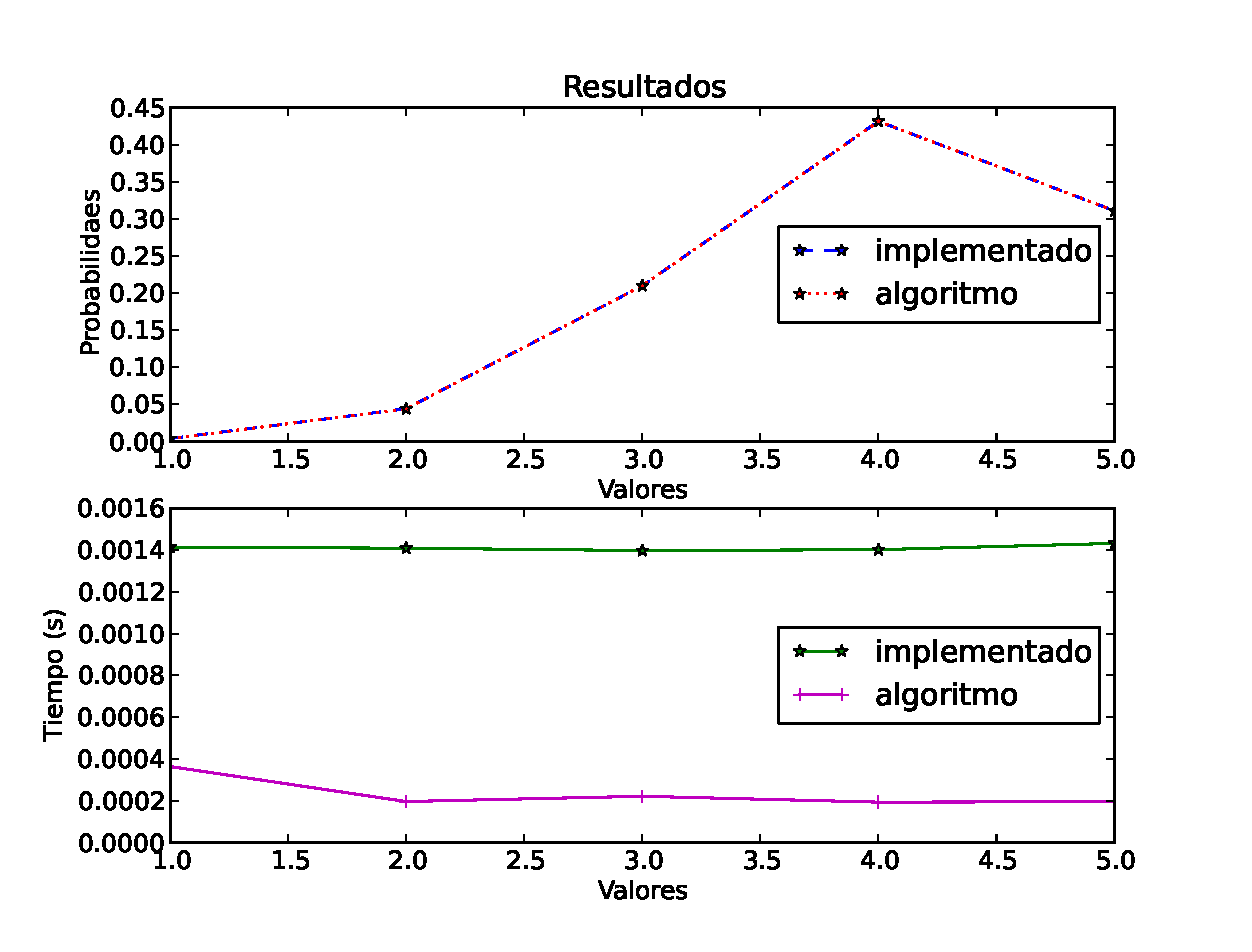
\includegraphics[width=1.1\textwidth]{grafica.eps}
\caption{Probabilidades y tiempo}
\end{figure}




\section{Análisis de los resultados}
En cualquiera de las muestras la función implementada tarda más en compilar el programa que el algoritmo ya que tiene que cargar más paquetes , comandos, etc. mientras que el algoritmo es muy básico y bastante eficaz.

Respecto a las probabilidades , dependiendo de los valores que se tomen, puede salir hasta exactamente igual en la función implementada que la creada. En la mayoría de casos, sale aproximada.
\chapter{Conclusiones}

En resumen, se definió las variables aleatorias y la función, se ha creado cuatro algoritmos sobre la función de distribución hipergeométrica, dos de ellos con ejemplos, uno genérico, y uno con la función implementada. Se ha creado un módulo para obtener el tiempo empleado en cada algoritmo y los errores de cálculo entre el programa implementado y el genérico.

Este informe detalla brevemente en lo que ha consistido el proyecto. En él, se ha identificado los propósitos del mismo.
Se ha recopilado información sobre la función de distribución hipergeométrica y se ha implementado este aspecto matemático en el lenguaje de programación de esta asignatura, Python.
Por último, se ha adquirido más destreza en el uso de programas como \LaTeX{} y Beamer para la creación de textos científicos.


\begin{appendix}
En este apéndice se incluirá los algoritmos Python que se han utilizado en el procedimiento experimental.
\chapter{Algoritmo Poker de Ases}
\begin{verbatim}
#!encoding:UTF-8
#!usr/bin/python

import math

def fact(p):
  a=1
  if p<0:
    return 0 
  elif p==0:
    return 1
  else:
    for i in range(2,p+1):
      a=a*i
  return (a)

N1=int(raw_input("Introduzca el número de ases de las baraja (N1 > x):"))
N2=int(raw_input("Introduzca el número de no ases en la baraja (N2 > n-x):"))
n=int(raw_input("Introduzca el número de cartas extraídas de la baraja (n < N1+N2) :"))
x=int(raw_input("Introduzca el número de ases en las 5 extracciones :"))
N = N1 + N2

comb1 = float(fact(N1)/(fact(x)*fact(N1-x)))
comb2 = float(fact(N2)/(fact(n-x)*fact(N2-n+x)))
comb3 = float(fact(N)/(fact(n)*fact(N-n)))

probabilidad = (comb1+comb2)/comb3
print "La probabilidad es : ", probabilidad
\end{verbatim}
\chapter{Algoritmo Color}
\begin{verbatim}
#!encoding:UTF-8
#!/usr/bin/python

import math

def fact(p):
    a=1
    if p<0:
        return 0
    elif p==0:
        return 1
    else:
        for i in range(2,p+1):
            a=a*i
    return (a)
        
N1=int(raw_input("Introduzca el número de cartas de determinado palo (N1 > x):"))
N2=int(raw_input("Introduzca el número de cartas de los otros tres palos (N2 > n-x):"))
n=int(raw_input("Introduzca el número de cartas extraídas de la baraja (n < N1+N2:"))
x=int(raw_input("Introduzca el número de cartas extraidas de un determinado palo :"))
N=N1+N2

comb1=float(fact(N1)/(fact(x)*fact(N1-x)))
comb2=float(fact(N2)/(fact(n-x)*fact(N2-n+x)))
comb3=float(fact(N)/(fact(n)*fact(N-n)))

probabilidad=(comb1*comb2)/comb3
print"La probabilidad es : ",probabilidad
\end{verbatim}
\chapter{Algoritmo F.D Hipergeométrica}
\begin{verbatim}
#!encoding:UTF-8
#!/usr/bin/python

import math
import time

start1 = time.time()
def fact(p):
    a=1
    if p<0:
        return 0
    elif p==0:
        return 1
    else:
        for i in range(2,p+1):
            a=a*i
    return (a)

finish1 = time.time() - start1     
        
A=int(raw_input("Introduzca el A (A>x): "))
B=int(raw_input("Introduzca el B (B>n-x): "))
n=int(raw_input("Introduzca el n: (n<A+B)"))
x=int(raw_input("Introduzca la x: "))

N=A+B

start2 = time.time()
comb1=float(fact(A)/(fact(x)*fact(A-x)))
comb2=float(fact(B)/(fact(n-x)*fact(B-n+x)))
comb3=float(fact(N)/(fact(n)*fact(N-n)))

probabilidad=(comb1*comb2)/comb3

print"La probabilidad es :",probabilidad

finish2 = time.time() - start2

finish = finish1 + finish2

print finish
\end{verbatim}
\chapter{F.D Hipergeométrica Implementada}
\begin{verbatim}
from scipy.stats import hypergeom
import numpy as np
import time

M=int(raw_input("Introduzca el valor de M: "))
n=int(raw_input("Introduzca el valor de n: "))
N=int(raw_input("Introduzca el valor de N: "))
x=int(raw_input("Introduzca el valor de x: "))
start = time.time()

rv = hypergeom(M, n, N)
pmf_cartas = rv.pmf(x)

print pmf_cartas

finish=time.time()-start

print finish
\end{verbatim}
\end{appendix}

\begin{thebibliography}{99}
\bibitem{}
Francisco Javier Martín-Pliego, José María Montero Lorezno,Luis Ruiz-Maya Pérez. Problemas de Probabilidad 
\bibitem{}
Guido Rossum. Python reference manual. Technical report, Amsterdam, The Netherlands, 1995.
\bibitem{}
Juan José Salazar y Marta López Yurda. Ejercicios Resueltos de probabilidad.
\bibitem{}
ACM LaTeX Style. $http://www.acm.org/publications/latex_style/.$
\end{thebibliography}
\ \\
\end{document}


